% Computer Physics Communications (Elsevier) submission version of the TorchFDTD manuscript.
% Maintained separately from the arXiv version in docs/paper/manuscript.tex.
% Template: Elsevier CPiP template (legacyfileshare.elsevier.com/promis_misc/cpc-cpip-template.tex), class elsarticle.
% Writing rules: no em dashes, no semicolons, no self-assessment adjectives.
\documentclass[preprint,11pt]{elsarticle}
% The preprint text block of elsarticle is narrower than the tables and the two-line Yee update, so the review
% copy uses 11 pt type on A4 with 25 mm margins. Elsevier typesets the accepted article in the journal layout.
\usepackage[a4paper,margin=25mm]{geometry}
\usepackage[T1]{fontenc}
\usepackage{lmodern}
\usepackage{amsmath}
\usepackage{amssymb}
\usepackage{graphicx}
\usepackage{booktabs}
\usepackage{xcolor}
\usepackage{listings}
\PassOptionsToPackage{obeyspaces}{url}
\usepackage{xurl}
\usepackage{hyperref}
\definecolor{citelink}{RGB}{0,90,160}
\hypersetup{colorlinks=true}
% elsarticle sets every link colour to blue at \begin{document}, so the colours are set after its hook
\AtBeginDocument{\hypersetup{citecolor=citelink, linkcolor=black, urlcolor=black, filecolor=black}}
\urlstyle{same}
\usepackage{lineno}
\biboptions{sort&compress}
\definecolor{codekw}{RGB}{36,49,59}
\definecolor{codecomment}{RGB}{107,116,128}
\lstset{language=Python, basicstyle=\small\ttfamily, keywordstyle=\bfseries\color{codekw},
  commentstyle=\itshape\color{codecomment}, stringstyle=\color{codekw}, columns=fullflexible,
  keepspaces=true, breaklines=true, showstringspaces=false, xleftmargin=1.2em,
  aboveskip=6pt, belowskip=6pt, captionpos=b, frame=none}
\newcommand{\code}[1]{{\small\nolinkurl{#1}}}
\newcommand{\micron}{\ensuremath{\mu\mathrm{m}}}
% Written by scripts/build_cpc.py from the labels of supplementary-cpc.tex. Do not edit.
\expandafter\def\csname si@aniso\endcsname{S1}
\expandafter\def\csname si@batch\endcsname{S2}
\expandafter\def\csname si@projection\endcsname{S3}
\expandafter\def\csname si@ports\endcsname{S4}
\expandafter\def\csname si@shape\endcsname{S5}
\expandafter\def\csname si@crosssolver\endcsname{S6}
\expandafter\def\csname si@tiling\endcsname{S7}
\expandafter\def\csname si@host\endcsname{S8}
\expandafter\def\csname si@scaling\endcsname{S9}
\expandafter\def\csname si@metagrating\endcsname{S10}
\expandafter\def\csname si@pillar\endcsname{S11}

\newcommand{\suppsec}[1]{Supplementary Section~\csname si@#1\endcsname}
\newcommand{\suppsecs}[2]{Supplementary Sections~\csname si@#1\endcsname{} and~\csname si@#2\endcsname}
% Items only the author can supply. scripts/build_cpc.py lists every \authorcheck left in the source.
\newcommand{\authorcheck}[1]{\textcolor{red}{#1}}
\setlength{\emergencystretch}{1.5em}
\renewcommand{\topfraction}{0.85}
\renewcommand{\bottomfraction}{0.8}
\renewcommand{\textfraction}{0.1}
\renewcommand{\floatpagefraction}{0.75}
% Generated from docs/validation/flux.json.
\newcommand{\SlabTError}{0.00153444}
\newcommand{\SlabRError}{0.00153535}
\newcommand{\SlabEnergyError}{4.43991\times10^{-6}}

% Generated from docs/validation/cross_solver_3060.json and the fastest docs/validation/cross_solver/meep_throughput_ranks*.json.
\newcommand{\CrossMeepRanks}{four}
\newcommand{\CrossSlabPairT}{1.6\times10^{-5}}
\newcommand{\CrossSpherePair}{0.7}
\newcommand{\CrossFdtdxStepMin}{4.4}
\newcommand{\CrossFdtdxStepMax}{5.7}
\newcommand{\CrossFdtdxFullMin}{6.4}
\newcommand{\CrossFdtdxFullMax}{7.3}
\newcommand{\CrossMeepFullMin}{30}
\newcommand{\CrossMeepFullMax}{36}
\newcommand{\CrossMeepStepMin}{36}
\newcommand{\CrossMeepStepMax}{41}
\newcommand{\CrossAdjointCheckpointRatio}{52}
\newcommand{\CrossAdjointReversibleRatio}{2.0}
\newcommand{\CrossGradientDiff}{1.1\times10^{-7}}

% Generated from docs/validation/paper_review/torchfdtd-precision-a100.json and docs/validation/cross_solver/meep_throughput_ranks*.json.
\newcommand{\PrecisionMeepRanks}{four}
\newcommand{\PrecisionRatioMin}{49}
\newcommand{\PrecisionRatioMax}{59}
\newcommand{\PrecisionSingleRatioMin}{77}
\newcommand{\PrecisionSingleRatioMax}{97}
\newcommand{\PrecisionDoubleCost}{1.6}


\journal{Computer Physics Communications}

\begin{document}

\begin{frontmatter}

\title{TorchFDTD: GPU-accelerated finite-difference time-domain simulation with discrete adjoints and host-streamed execution for photonic inverse design}

\author[cnu]{Hyoseok Park\corref{cor1}}
\cortext[cor1]{Corresponding author.\\\textit{E-mail address:} phs137@o.cnu.ac.kr}
\address[cnu]{Department of Physics, Chungnam National University, Daejeon 34134, Republic of Korea}

\begin{abstract}
Gradient-based photonic design needs full-wave derivatives with respect to millions of parameters, but on one GPU workstation the time-domain adjoint is limited by device memory and by the incompatibility of fused update kernels with automatic differentiation. We present TorchFDTD, an open-source finite-difference time-domain (FDTD) package that addresses both limits. Its Yee, absorber and dispersion updates execute as fused CUDA kernels captured in a CUDA graph, and every kernel is paired with a transpose kernel derived from its update, so material and geometry derivatives are obtained by a discrete adjoint that PyTorch chains with differentiable objectives. For problems that exceed the device, a streamed mode advances the domain one causal slab at a time and keeps the global state and checkpoints in host memory without changing the discretization. We validate the package against analytic solutions, Meep, FDTDX, a rigorous coupled-wave solver, automatic differentiation and finite differences. On an A100 the fused path completes full forward solves of eight scenes 9.0 to 17.1 times faster than the PyTorch FDTD package it extends, and its double-precision solves are 49 to 59 times faster than those of Meep on a workstation CPU. On an eight-core workstation, streaming lowers the device allocation of a $256^3$ adjoint by 56\% at 4.1 to 4.8 times the resident time. A 54-million-cell pillar-array lens coupled to an angular-spectrum objective yields an adjoint derivative within 0.78\% of a central difference. The time-domain adjoint of a device with tens of millions of cells thus becomes available on one workstation GPU.
\\

\noindent \textbf{PROGRAM SUMMARY}

\begin{small}
\noindent
{\em Program Title:} TorchFDTD\\
{\em CPC Library link to program files:} (to be added by Technical Editor)\\
{\em Developer's repository link:} \url{https://github.com/hyoseokp/TorchFDTD}\\
{\em Licensing provisions:} MIT\\
{\em Programming language:} Python 3.10 or later, with CUDA C++ kernels compiled at run time through CuPy and a JavaScript browser workbench\\
{\em Supplementary material:} Supplementary Material with further validation, the data behind the figures and details of the design examples\\
{\em Nature of problem:} Gradient-based design of nanophotonic devices requires a full-wave Maxwell solver that returns broadband observables and their derivatives with respect to millions of material or geometry parameters. On a single workstation the time-domain adjoint is limited by GPU memory, because the backward sweep needs the forward field history and the working field state must fit the device. A second limit is the incompatibility between fused CUDA update kernels and framework automatic differentiation.\\
{\em Solution method:} The Yee scheme with convolutional perfectly matched layers, auxiliary-differential-equation dispersion and anisotropic tensors runs as two fused CUDA kernels per step inside a CUDA graph. Each kernel has a transpose kernel derived from its update, and the discrete adjoint is exposed to PyTorch as a custom autograd function so that geometry parameterizations, objectives built from the supported observations and optimizers are ordinary Torch code. Forward states for the transposed sweep come from binomial checkpoint replay or time reversal. A host-streamed mode partitions the domain into causal slabs with halos, advances one slab for $K$ steps on the device and keeps the global state and checkpoints in host memory. Guided-mode sources and monitors, total-field/scattered-field boxes, near-to-far projection, angular-spectrum propagation, GDSII import and process-level or tensor batches are provided.\\
{\em Additional comments including restrictions and unusual features:} Fused kernels require an NVIDIA GPU with CuPy, and a CPU path executes the same discrete operators for reference. Host streaming keeps full-domain state banks in host memory, so host capacity and device--host bandwidth bound the usable problem size and speed. Independent lateral tiling is an approximation that changes the boundary-value problem and is reported with its error against a full-domain solution. Multi-GPU execution of one domain is not part of this release.
\end{small}
\end{abstract}

\begin{keyword}
finite-difference time-domain \sep adjoint method \sep inverse design \sep GPU computing \sep PyTorch \sep metasurfaces \sep nanophotonics
\end{keyword}

\end{frontmatter}

\linenumbers

\section{Introduction}

The finite-difference time-domain (FDTD) method advances Maxwell's equations on a staggered grid and returns broadband observables from a single run \citep{yee1966,taflove2005}. Absorbing layers \citep{berenger1994,roden2000}, auxiliary differential equations for dispersive media \citep{okoniewski1997} and subpixel material averaging \citep{farjadpour2006} made it the standard full-wave solver of nanophotonics, and packages such as Meep \citep{oskooi2010} and commercial tools \citep{lumerical,tidy3d} expose it through scripting interfaces. Inverse design changed what is asked of the solver. Adjoint sensitivities turn one additional simulation into the gradient of an objective with respect to millions of design variables \citep{georgieva2002,jensen2011,elesin2012,piggott2015,molesky2018,hughes2018,christiansen2021}, and design frameworks built on frequency-domain solvers \citep{su2020,minkov2020} or on hybrid time and frequency-domain evaluation \citep{hammond2022} made that gradient central to nanophotonic design. The practical question became how to obtain it quickly on the hardware that a design group owns. Automatic differentiation of a Maxwell solver written in a machine-learning framework answers part of that question \citep{hughes2019}. The Fourier modal solver TORCWA showed that a PyTorch implementation makes rigorous coupled-wave gradients available to ordinary optimizers on a graphics processor \citep{kim2023}. GPU time-domain solvers such as fdtd-z moved the Yee update itself onto the device \citep{fdtdz}, and FDTDX brought reverse-mode differentiation and multi-GPU sharding to time-domain simulation in JAX \citep{mahlau2024}.

Two costs remain for the time-domain adjoint on a single workstation. The first is memory. The backward sweep needs the forward field history, and time-reversible reconstruction or checkpoint replay trades retained history against recomputation \citep{griewank2000,mahlau2024,mahlau2026}. However, even with that history under control, a resident implementation must hold the complete working state on the device. For a $10^9$-cell grid in single precision the six field components alone occupy 24~GB, and the adjoint sweep adds a cotangent state of equal size and at least one checkpoint, so the working state exceeds 70~GB before the material arrays and absorber memories are counted. That approaches the 80~GB of the A100 and exceeds the 12~GB of the RTX 3060 used in this work. The second cost is the interaction between differentiation and kernel fusion. Framework automatic differentiation records every array operation, so the fused update kernels that give an FDTD code its speed cannot participate in the graph unless they are supplied with their own derivative rules.

Here, we address both costs in TorchFDTD. Its Yee, absorber and dispersion updates run as fused CUDA kernels captured in a CUDA graph. Instead of letting the framework record these updates, we give each kernel its own derivative rule, a transpose kernel derived from the discrete update. The discrete adjoint is therefore exposed to PyTorch as a custom autograd function and chains with Torch geometry parameterizations, optimizers and differentiable objectives built from the supported observations. We partition the field state into causal slabs, strips of the domain padded by halos as wide as the number of steps advanced per block. A streamed mode advances one slab at a time on the device while the global state and the checkpoints reside in host memory (Fig.~\ref{fig:overview}). The device allocation then follows the width of one slab rather than the length of the domain along the partitioned axis, although it still grows with the transverse cross-section. The discrete problem is unchanged. Guided-mode ports, total-field/scattered-field boxes, near-to-far projection, angular-spectrum propagation to remote observation planes, GDSII import and a browser workbench connect the solver to a complete design workflow. The grid and backend foundation come from the MIT-licensed \code{flaport/fdtd} package \citep{fdtd}, and PyTorch supplies device arrays, graph capture and the optimizer interface \citep{paszke2019}.

\begin{figure}[tbp]
\centering

\includegraphics[width=\linewidth]{figures/execution-overview.pdf}
\caption{Execution and differentiation in TorchFDTD. (a) The forward map from design parameters to an objective evaluated after angular-spectrum propagation, and its transposed chain. Every forward kernel has its own transpose kernel, and the transposed sweep obtains forward states from checkpoint replay. (b) Host-streamed execution sweeps causal slabs of $W$ cells with halos of $K$ cells over blocks of $K$ steps. One slab block resides on the GPU while the state banks of all slabs and the block checkpoints stay in host DRAM. (c) Independent lateral tiles solve overlapping subdomains with their own absorbers and assemble the core fields on the output plane. Coupling across the artificial cut is lost, and the resulting error is measured against a full-domain solution.}
\label{fig:overview}
\end{figure}

On an A100 the fused path completes full forward solves of the tested scenes 9.0 to 17.1 times faster than the package it extends, and in double precision its solves of a dielectric sphere are \PrecisionRatioMin{} to \PrecisionRatioMax{} times faster than those of Meep on a workstation CPU. Host streaming is meant for problems whose resident allocation exceeds the device. On an eight-core workstation it lowers the peak device allocation of a $256^3$ adjoint by 56\% at 4.1 to 4.8 times the resident time, and on the RTX 3060 this factor falls from 4.7 to 2.7 as the grid grows from $128^3$ to $320^3$.

This paper describes the numerical method (Section~\ref{sec:formulation}), the discrete adjoint (Section~\ref{sec:adjoint}), the execution modes (Section~\ref{sec:execution}) and the software structure with usage examples (Section~\ref{sec:software}). Section~\ref{sec:validation} validates the package against analytic solutions, independent solvers and finite differences, Section~\ref{sec:performance} reports throughput, its scaling with grid size and the memory--time trade-off of host streaming, and Section~\ref{sec:examples} presents a complete metagrating design and a propagated optical objective on a workstation. The Supplementary Material collects further validation, the data behind the figures and details of the design examples.

\section{Numerical method}
\label{sec:formulation}

\subsection{Yee update and time step}

The six field components occupy the standard staggered positions \citep{yee1966}. In a nonmagnetic medium the reduced update reads
\begin{equation}
E^{n+1}=E^{n}+S\,\epsilon^{-1}\,\mathcal{C}^{-}\!\left(H^{n+1/2}\right)+s^{n+1},\qquad
H^{n+3/2}=H^{n+1/2}-S\,\mathcal{C}^{+}\!\left(E^{n+1}\right)+m^{n+3/2},
\label{eq:yee}
\end{equation}
where $S=c\Delta t/h$ with $h$ the smallest mesh step, $\mathcal{C}^{\pm}$ are the forward and backward difference curls scaled by the local metric, and $s$ and $m$ are soft electric and magnetic source increments added after the corresponding update. Fields start from zero, the first recorded electric sample lies at $\Delta t$ and the first magnetic sample at $3\Delta t/2$, and every Fourier transform in the package keeps that half-step offset. For $d$ active dimensions with minimum primal widths $h_a$ the time step is bounded by
\begin{equation}
\Delta t\leq\frac{\eta}{c\sqrt{\sum_{a=1}^{d}h_a^{-2}}},\qquad 0<\eta\leq0.99,
\label{eq:cfl}
\end{equation}
which reduces to $\eta h/(c\sqrt{d})$ on a uniform mesh. A graded rectilinear mesh keeps this fine-grid step, so coarsening the background reduces the cell count at a fixed physical duration without local time stepping. The two-dimensional solver suppresses the $z$ derivatives while keeping all six components, and Bloch problems carry complex fields.

\subsection{Boundaries}

Convolutional perfectly matched layers \citep{roden2000} store one memory variable per transverse derivative inside each absorbing face. The stretching coefficients $\kappa$, $\sigma$ and $\alpha$ follow polynomial profiles configured per face, so opposite faces and neighboring faces of different type may carry different depths and gradings. Periodic and Bloch pairs wrap the difference operators without a duplicated end plane, and the Bloch phase enters through the wrapped stencil. Perfect electric conductor faces and electric antisymmetry planes hold the tangential electric field at zero on the boundary node. Perfect magnetic conductor and magnetic symmetry faces need the dual arrangement, in which the upper boundary node of each tangential electric component becomes a stored degree of freedom. The package carries those face arrays through the resident, streamed and batched paths, through their checkpoints, and through the absorber memories of neighboring faces. Any face type may adjoin any other, so \suppsec{aniso} measures the reflection of an absorbing face next to a magnetic wall.

\subsection{Materials and geometry}

A nondispersive cell carries a real permittivity at each Yee electric position. Dispersive materials add up to sixteen Drude or Lorentz poles integrated with the trapezoidal auxiliary differential equation of \citet{okoniewski1997}, and measured refractive-index tables are fitted to a passive multipole model whose error and band are reported before the fit is accepted. Anisotropic media \citep{oskooi2009} use a symmetric positive-definite permittivity tensor sampled at grid nodes and applied to the curl through the node assembly $S=D^{-1/2}\bigl(\tfrac18\sum R^{\dagger}\epsilon^{-1}R\bigr)D^{-1/2}$, with the tensor restricted to eigenvalues at or above one so that the vacuum time step of Eq.~\eqref{eq:cfl} remains admissible. Inside an absorbing face a tensor is admitted only when the face normal is a principal axis with a non-intermediate eigenvalue, because the stretched-coordinate layer is unstable otherwise \citep{becache2003}, and \suppsec{aniso} gives the criterion and the spectral radii of admitted and rejected tensors.

Geometry enters through analytic solids (boxes, cylinders, spheres, ellipsoids, rings and extruded polygons with holes) placed by an ordered rotation and a pivot, with a lower mesh order winning overlaps. Membership is evaluated only inside a conservative axis-aligned support, and an optional dielectric subpixel operator averages the permittivity across interfaces \citep{farjadpour2006}. GDSII layouts map layer and datatype pairs to extrusion intervals and materials, apply Boolean etch layers, staircase a sidewall angle on the native $z$ nodes and keep polygon holes with even-odd filling \citep{gdstk}.

\subsection{Sources, monitors and projections}

Point and sheet sources inject Gaussian, ramped continuous or sampled waveforms with Cartesian or angular polarization. A one-way plane covering a periodic transverse cell injects a normally incident wave without a backward component, and a closed total-field/scattered-field box \citep{schneider2010} surrounds an isolated scatterer with an incident field that is corrected on its faces. Guided-mode sources solve the full-vector finite-difference eigenproblem of the port cross-section \citep{zhu2002} at the temporal wavenumber $\tilde k_0=2\sin(\omega\Delta t/2)/(c\Delta t)$, convert the eigenvalue to the longitudinal Yee propagation constant $\beta=2\arcsin(\tilde\beta\,\Delta w/2)/\Delta w$, and inject electric and magnetic Huygens sheets at their staggered positions and times. The eigensolver returns a canonical basis for degenerate polarization pairs by diagonalizing the overlap of their transverse components, so a port's mode index is stable across machines.

Point monitors record one component per step. Plane monitors accumulate six-component complex spectra with the Yee interpolation and the magnetic half-step phase applied before the signed Poynting flux is formed, and flux ratios are taken against a matching reference run. A closed six-face box of stored spectra feeds a near-to-far transform of the equivalent surface currents \citep{luebbers1991} in the asymptotic form and in a finite-distance form built on the free-space dyadic Green function. The transform accepts angular, spherical, Cartesian and direction-cosine observation sets and a complex passive exterior index that may vary per frequency, and an open-surface variant projects from one to five faces with an edge window. Periodic cells return Bloch diffraction orders separated into forward and backward propagating branches.

\section{Discrete adjoint}
\label{sec:adjoint}

\subsection{Transposed updates}

Let $u^{n}$ collect the field, absorber and polarization state after step $n$, and let the forward step be $u^{n+1}=F_n(u^{n},p)$ with parameters $p$. For an objective $J(u^{N},\ldots)$ the reverse recursion
\begin{equation}
\bar u^{n}=\left(\frac{\partial F_n}{\partial u}\right)^{\!\mathsf T}\bar u^{n+1}+\frac{\partial J}{\partial u^{n}},\qquad
\bar p=\sum_n\left(\frac{\partial F_n}{\partial p}\right)^{\!\mathsf T}\bar u^{n+1},
\label{eq:adjoint}
\end{equation}
returns the gradient of $J$ with respect to every parameter after one backward sweep. Each transpose is a separate kernel that mirrors its forward kernel. The Yee curls transpose to the opposite-direction differences with the same metric. The absorber recursion transposes to $\bar\psi_{\mathrm{mem}}=\bar\psi+\bar y$, $\bar D=\kappa^{-1}\bar y+c\,\bar\psi_{\mathrm{mem}}$ and $\bar\psi_{\mathrm{old}}=b\,\bar\psi_{\mathrm{mem}}$ for the memory variable $\psi$ with coefficients $b$ and $c$, and the trapezoidal dispersion update transposes to the same two-by-two system applied to the cotangents. The material cotangent $\bar\epsilon^{-1}$ accumulates the product of the electric cotangent with the curl at every step.

A chain of differentiable material producers maps that cotangent onto design variables. The variables may be a scalar or tensor permittivity per cell, a density field passed through a physical-radius filter, symmetry averaging and a smooth projection \citep{lazarov2011,wang2011}, an analytic solid whose occupancy is a smooth signed-distance step of fixed physical width, a polygon or spline outline whose vertices or control points move that step, or a source waveform. Objectives may combine point signals, plane spectra, the amplitudes of guided modes at any number of ports and the far or near-zone fields of a projected box, since each observation is linear in the stored fields and carries its own transpose. Because the transposed sweep is wrapped as a Torch autograd function, everything upstream of the permittivity and downstream of the observations remains ordinary differentiable Torch code.

\subsection{Checkpoint replay and reversibility}

Retaining $u^{n}$ for every time step scales with both volume and duration, so the backward sweep instead replays the forward pass between checkpoints. With $C$ checkpoints and $N$ steps the binomial schedule of \citet{griewank2000} minimizes the number of recomputed steps, and the checkpoints are placed in GPU or host memory according to the execution policy. A retained backward pass keeps the adjoint state between transposes, so several objectives can be differentiated from one forward run. For lossless nondispersive periodic problems an opt-in reversible mode reconstructs the forward fields by stepping Eq.~\eqref{eq:yee} backward, in the spirit of \citet{mahlau2024}, and the absorbing-face variant records the fields at the interface between interior and absorber so that the interior reconstruction stays lossless while the absorber is replayed. Which mode is admissible follows from the material and boundary content of the project rather than from a user setting.

\section{Execution on a workstation}
\label{sec:execution}

\subsection{Fused kernels and batches}

One simulation on the device runs as a sequence of fused kernels compiled through CuPy \citep{okuta2017}: one kernel updates all electric components together with the absorber memories of every face, and one kernel updates the magnetic components. The kernels are captured once into a CUDA graph together with source injection and monitor accumulation, so a run of $N$ steps replays $N$ graph launches without Python in the loop \citep{paszke2019}. The CPU path executes the same discrete operators with NumPy and Torch tensors and serves as the reference for every device test.

A design loop evaluates many structures, so the package also runs them as separate processes on one or more devices or as one tensor batch of compatible structures, and a seeded differential-evolution optimizer \citep{storn1997} drives either level for gradient-free design (\suppsec{batch}).

\subsection{Host-streamed slabs}
\label{sec:streaming}

The streamed mode partitions the domain along $x$ into slabs of $W$ cells and advances each slab for $K$ steps before moving to the next, so a block of $K$ steps needs a halo of $K$ cells on either side of the slab (Fig.~\ref{fig:overview}b). Only the slab under update, its halos and its checkpoint reside on the device. The remaining field state lives in banks, contiguous buffers in host DRAM that are read into and written from the device slab by slab. The transposed sweep runs this tiling in reverse, and both sweeps see the same number of field updates plus the halo overhead $2K/W$ per block. Absorber memories, dispersion states and the stored magnetic-wall faces travel with their slabs, and the slab whose core ends at the upper boundary owns the face arrays. Because the halos carry the complete state that the Yee stencil needs at every block, the streamed sweep reproduces the resident discrete problem up to floating-point ordering.

A policy is admitted only after accounting for the active device workspace, the global state banks, the checkpoints, the material tensors and the observation buffers. Slab width $W$ and temporal depth $K$ control the active field extent $W+2K$, while the checkpoint count controls retained history and replay work. For a domain of $N_x\times N_y\times N_z$ cells partitioned along $x$, the device workspace therefore scales with $(W+2K)N_yN_z$ rather than with $N_xN_yN_z$, so it still grows with the transverse cross-section. The host allocation scales with the full volume plus the retained checkpoints, and host capacity and device--host bandwidth bound the usable policies.

\subsection{Exterior propagation and lateral tiling}
\label{sec:hybrid}

A separate interface partitions a planar device into independently solved, overlapping lateral tiles, each with its own absorber and output plane, and assembles their core fields on the global plane (Fig.~\ref{fig:overview}c). In contrast to the causal slabs above, this is an overlapping-domain approximation of the kind used for large-area metasurfaces \citep{pestourie2018,lin2019}, and it changes the boundary-value problem. A neighboring-tile mismatch is reported as a diagnostic, and Section~\ref{sec:hybrid-validation} measures the error against a full-domain solution.

In a homogeneous, lossless and source-free exterior containing outgoing waves, a recorded plane field is propagated with the angular spectrum \citep{goodman2005},
\begin{equation}
u(x,y,z_0+d)=\mathcal{F}^{-1}_{xy}
 \left[\mathcal{F}_{xy}\{u(x,y,z_0)\}
 \exp\!\left(\mathrm{i}d\sqrt{k^2-k_x^2-k_y^2}\right)\right],
\qquad d\geq0,
\label{eq:asm}
\end{equation}
where the square-root branch makes evanescent components decay. The implementation propagates the sampled electric and magnetic components rather than a scalar transmission coefficient, and zero padding limits the periodic wraparound of the discrete transform \citep{matsushima2009}. The interface returns selected planes, axial sections or points without storing an exterior volume. For a tiled plane $u=\sum_j R_j u_j(p)$ with fixed assembly maps $R_j$, the reverse operation applies $R_j^{\mathsf T}$ to the global plane cotangent before the local FDTD adjoint, and the propagation of Eq.~\eqref{eq:asm} has a differentiable transpose, so an exterior intensity objective differentiates to the material parameters.

\section{Software structure and usage}
\label{sec:software}

TorchFDTD is a Python package of about 36\,000 lines with a serializable scene model, a solver core, an adjoint layer and a browser workbench. A \code{Project} holds the region, materials, structures, sources, monitors and execution policy, and it round-trips through JSON so that the workbench, the command line and scripts operate on one description. The solver core contains the fused CUDA kernels and their transposes, the streamed executor, the batch runners and the CPU reference path. The adjoint layer wraps the transposed sweep as Torch autograd functions and provides the material producers, mode-port and projection objectives, memory estimation and checkpoint tiers. The workbench is a FastAPI service with a JavaScript client for scene editing, execution, field inspection and GDSII import. Optional extras add CuPy for the fused kernels, gdstk for layouts and h5py for HDF5 output, and the repository carries 1551 tests that exercise the CPU path everywhere and the CUDA path where a device is present.

Listing~\ref{lst:forward} runs a three-dimensional waveguide with a fused CUDA solve and saves the result. Lengths are in micrometers.
\begin{lstlisting}[float=tbp,caption={A forward simulation with the fused CUDA path.},label={lst:forward}]
from torchfdtd import (Project, Region, Structure, Source, Monitor,
                       Simulation)

project = Project(
    name="My waveguide",
    region=Region(dimension="3d", size=(8, 6, 2), mesh=0.05, steps=1000,
                  backend="cuda", cuda_kernel="fused"),
    structures=[Structure(name="core", size=(8, 0.65, 0.4))],
    sources=[Source(center=(-2.5, 0, 0), wavelength=1.55)],
    monitors=[Monitor(name="output", center=(2, 0, 0))],
)
project.save("project.json")          # opens in the browser workbench
result = Simulation(project).run()
result.save("results/run.npz")
\end{lstlisting}

Listing~\ref{lst:adjoint} differentiates a point-signal objective with respect to the radius of a smooth sphere. The permittivity is built by a differentiable producer from a Torch parameter, the differentiable simulation replays four host checkpoints during the transposed sweep, and a standard optimizer consumes the gradient. Replacing \code{AdjointOptions} by a streamed policy with a slab width and temporal depth switches this model to host-streamed execution.
\begin{lstlisting}[float=tbp,caption={A differentiable simulation with checkpoint replay.},label={lst:adjoint}]
import torch
from torchfdtd import (Project, Region, Source, Monitor, AdjointOptions,
                       DifferentiableSimulation, smooth_sphere_epsilon)

project = Project(
    region=Region(size=(1.6, 1.5, 1.4), mesh=0.1, pml_cells=3, steps=40,
                  precision="float64"),
    sources=[Source(center=(-0.2, 0, 0), pulse="continuous",
                    wavelength=1.1)],
    monitors=[Monitor(center=(0.1, 0, 0))],
)
radius = torch.nn.Parameter(
    torch.tensor(0.25, device="cuda", dtype=torch.float64))
model = DifferentiableSimulation(
    project, AdjointOptions(checkpoints=4, storage="host",
                            host_budget_bytes=128 * 1024**2))
optimizer = torch.optim.Adam([radius], lr=0.003)
optimizer.zero_grad()
epsilon = smooth_sphere_epsilon(project.region, radius, inside=3.0, width=0.09)
result = model(epsilon)
loss = result.signals[:, 0].square().mean()
loss.backward()
optimizer.step()
\end{lstlisting}

\section{Validation}
\label{sec:validation}

\subsection{Analytic references}

A lossless slab of index 1.5 and thickness 0.2~\micron{} in air, excited by a broadband sheet in a periodic two-dimensional cell with a 0.025~\micron{} mesh and 16 absorbing cells at each end, is compared with the normal-incidence transmission
\begin{equation}
T(\lambda)=\left[1+\left(\frac{n^{2}-1}{2n}\right)^{2}\sin^{2}\!\left(\frac{2\pi nd}{\lambda}\right)\right]^{-1},\qquad R=1-T,
\label{eq:slab}
\end{equation}
at 31 wavelengths between 1.3 and 1.8~\micron{}. The plane-monitor spectra reach maximum absolute errors of \SlabTError{} in transmission and \SlabRError{} in reflection, and the residual $R+T-1$ stays below $\SlabEnergyError$ (Fig.~\ref{fig:flux-validation}). The transmission and reflection errors are equal and opposite and three orders of magnitude above the energy residual, so the remaining error lies in the discrete response of the slab rather than in the flux monitors.

\begin{figure}[tbp]
\centering

\includegraphics[width=\linewidth]{figures/flux-validation.pdf}
\caption{Plane-monitor spectra of the lossless slab. (a) The two-dimensional cell, periodic along $y$, with the slab, the source plane, the reflection (R) and transmission (T) monitors and the absorbing layers, to scale along $x$. (b) Transmission and reflection of the 31 recorded samples, with Eq.~\eqref{eq:slab} as the solid line. (c) Absolute errors of both spectra and the energy residual $|R+T-1|$ on a logarithmic axis.}
\label{fig:flux-validation}
\end{figure}

A closed total-field/scattered-field box around a dielectric sphere yields the scattering cross-section over nine wavelengths, which is compared with the Mie series \citep{bohren1983}. The error is set by the staircased sphere surface rather than by the box or the duration, and it is not monotonic in the mesh. It falls from 8.9\% at a 0.1~\micron{} mesh to 0.31\% at 0.05~\micron{}, rises to 1.05\% at 0.025~\micron{} and falls again to 0.55\% at 0.02~\micron{}, while doubling the physical duration leaves the 0.025~\micron{} value unchanged (Table~\ref{tab:tfsf-sphere}, Fig.~\ref{fig:tfsf-sphere}). Cross-sections of this sphere are therefore accurate to about one percent from a 0.05~\micron{} mesh onward, where the staircase, not the resolution, limits the error.

% Generated by scripts/build_paper_assets.py from native validation JSON.
\begin{table}[tbp]
\centering
\small
\renewcommand{\arraystretch}{1.15}
\caption{Closed-box TFSF sphere scattering on RTX 5880. The maximum relative cross-section error is taken over nine wavelengths. Physical domain and PML thickness stay fixed. The final row doubles the physical duration. The error sequence is not monotonic.}
\label{tab:tfsf-sphere}
\begin{tabular}{@{}lrrrr@{}}
\toprule
$h$ ($\mu$m) & Grid & \shortstack{Time\\(fs)} & \shortstack{Max error\\(\%)} & \shortstack{Empty box\\($\mu$m$^2$)} \\
\midrule
0.1 & $32^3$ & 120 & 8.8963 & $6.68\times10^{-15}$ \\
0.05 & $64^3$ & 120 & 0.3086 & $1.11\times10^{-14}$ \\
0.025 & $128^3$ & 120 & 1.0474 & $2.19\times10^{-15}$ \\
0.02 & $160^3$ & 120 & 0.5514 & $1.37\times10^{-14}$ \\
0.025 & $128^3$ & 240 & 1.0474 & $2.32\times10^{-15}$ \\
\bottomrule
\end{tabular}
\end{table}


\begin{figure}[tbp]
\centering

\includegraphics[width=\linewidth]{figures/tfsf-sphere.pdf}
\caption{Scattering cross-section of the dielectric sphere from the closed total-field/scattered-field box at four mesh steps. (a) Section $z=0$ of the scene: the sphere inside the total-field region (orange), the closed scattered-field flux surface (teal) and the absorbing layer (grey), with the incident direction and polarization. (b) Recorded cross-sections with the Mie series as reference. (c) Relative error against the Mie series at the nine recorded wavelengths.}
\label{fig:tfsf-sphere}
\end{figure}

Dispersive and lossy media are checked on a Drude slab of thickness 0.1~\micron{} and a two-pole Lorentz slab of thickness 0.5~\micron{} at normal incidence, against the transfer-matrix reflection, transmission and absorption of the permittivity used in the solver (Fig.~\ref{fig:dispersive}). At a 20~nm mesh the largest errors in $R$, $T$ and $A$ over 21 wavelengths between 1.3 and 1.8~\micron{} are $1.1\times10^{-3}$ for the Drude slab and $2.7\times10^{-3}$ for the Lorentz slab, in both polarizations, and halving the mesh lowers them to $2.7\times10^{-4}$ and $6.7\times10^{-4}$, a factor of four. Passing the permittivity through the passive multipole fit of Section~\ref{sec:formulation} changes these quantities by less than $2.9\times10^{-9}$. The trapezoidal auxiliary differential equation reproduces lossy dispersive responses with second-order accuracy, and absorptions up to 0.24 are resolved to about $10^{-4}$ on the finer mesh.

\begin{figure}[tbp]
\centering

\includegraphics[width=\linewidth]{figures/dispersive-slabs.pdf}
\caption{Dispersive slabs at normal incidence. (a) The two slabs in their periodic cells, to scale along $x$, with the source plane, the reflection (R) and transmission (T) points and the absorbing layers. (b) Drude slab of thickness 0.1~\micron{} and (c) two-pole Lorentz slab of thickness 0.5~\micron{}, with reflection, transmission and absorption from TorchFDTD at a 10~nm mesh (markers) and from the transfer-matrix solution (lines). (d) Largest absolute error of $R$, $T$ and $A$ over the band at two mesh steps, with a second-order guide.}
\label{fig:dispersive}
\end{figure}

Radiation projections of an electric dipole reproduce the closed-form fields from just outside the box to the far field, with errors that fall at second order to $2.8\times10^{-4}$ at 56 samples per face axis (\suppsec{projection}).

Guided-mode ports, anisotropic media and magnetic walls adjoining absorbers are validated in \suppsecs{aniso}{ports}. The ports are reciprocal and symmetric to $2\times10^{-3}$ or better, birefringent transmission is accurate to about one percent, and a magnetic symmetry plane adjoins an absorber at a reflection cost below $4\times10^{-4}$ of the incident power.

\subsection{Gradient checks}

We compare every differentiable path with full Torch automatic differentiation on a small grid and with central differences along a random direction, and we require the Taylor remainder of the directional derivative to fall quadratically. Table~\ref{tab:gradients} lists the agreement, and the double-precision autograd comparisons differ at the round-off level. On the $256^{3}$ problem of Section~\ref{sec:performance} the host-streamed material gradient agrees with the resident gradient to a relative $L_2$ difference of $3.3\times10^{-7}$ for the dielectric and $2.0\times10^{-7}$ for the two-pole material, both in single precision. The transposed kernels therefore reproduce the derivative of the discrete forward model to round-off in double precision and to a few parts in $10^{7}$ in single precision, in resident and streamed execution alike.

\begin{table}[tbp]
\centering
\small
\renewcommand{\arraystretch}{1.15}
\caption{Recorded gradient agreement of the discrete adjoint. Relative errors compare the transposed sweep with full Torch automatic differentiation unless a finite-difference (FD) reference is named. FP64 on CPU unless stated.}
\label{tab:gradients}
\setlength{\tabcolsep}{3pt}
\begin{tabular}{@{}llr@{}}
\toprule
Path & Reference & Relative error \\
\midrule
Polygon solid, checkpointed adjoint & autograd, CUDA FP32 & $1.2\times10^{-7}$ \\
Magnetic-wall faces with CPML & autograd & $2\times10^{-16}$ \\
Dispersive faces, four pole parameters & autograd & $2.7\times10^{-16}$ \\
Polygon vertices, voxel VJP & central FD, CPU and CUDA & $6.7\times10^{-8}$ \\
Polygon vertices through the solver & central FD & $4.4\times10^{-9}$ to $5.5\times10^{-8}$ \\
Spline control points & central FD & $1.8\times10^{-8}$ \\
Modal $|S_{21}|^{2}$ objective, N ports & autograd, CPU and CUDA & $1.3\times10^{-15}$ to $5.4\times10^{-15}$ \\
Far-field intensity objective & central FD & $3.4\times10^{-10}$ \\
Near-zone Poynting objective & central FD & $2.7\times10^{-9}$ \\
Streamed versus resident, tensor media & resident sweep & $1\times10^{-10}$ \\
Streamed versus resident, magnetic walls & resident sweep & $3\times10^{-7}$ \\
\bottomrule
\end{tabular}
\end{table}

The vertex derivative of a staircased shape converges to the physical shape derivative with the mesh and comes within 2\% of it at a 0.02~\micron{} mesh on a pentagon grating (\suppsec{shape}).

\subsection{Comparison with Meep, FDTDX and a rigorous coupled-wave solver}
\label{sec:cross-solver}

To compare the package with independent implementations, we ran Meep 1.34 \citep{oskooi2010} on the i7-12700 CPU and FDTDX 0.6.2 \citep{mahlau2024} on the RTX 3060 of the same workstation. The fixtures are the slab above, a Mie sphere at a 0.05~\micron{} mesh, and the vacuum and sphere scenes of Table~\ref{tab:open-source} at $64^{3}$ and $96^{3}$ cells. The absorbing layers share only their thickness, since FDTDX grades its convolutional profile differently and Meep uses a stretched-coordinate layer. Only TorchFDTD closes a total-field/scattered-field box around the sphere, so the other two subtract an empty run from total-field planes. Meep runs in double precision and the GPU solvers in single precision. Between any two solvers the slab transmission differs by at most $\CrossSlabPairT$ and the sphere cross-sections by at most \CrossSpherePair\% (Table~\ref{tab:cross-solver-accuracy}). The three codes agree more closely with each other than with the analytic slab response, so the remaining slab error belongs to the shared Yee discretization rather than to any one implementation.

On that device the fused engine steps \CrossFdtdxStepMin{} to \CrossFdtdxStepMax{} times faster than FDTDX and completes a solve \CrossFdtdxFullMin{} to \CrossFdtdxFullMax{} times faster, and against Meep on \CrossMeepRanks{} MPI ranks, its fastest setting on the CPU, the full solve is \CrossMeepFullMin{} to \CrossMeepFullMax{} times faster (Table~\ref{tab:cross-solver-speed}). For a periodic dielectric slab at $64^{3}$ cells and 128 steps the checkpointed sweep returns the permittivity gradient \CrossAdjointCheckpointRatio{} times faster than the FDTDX checkpointed method with the same two checkpoints and \CrossAdjointReversibleRatio{} times faster than its reversible method, and the gradients agree to a relative $L_2$ difference of $\CrossGradientDiff$. Against FDTDX the stepping ratio is smaller than the full-solve ratio, so part of the gain comes from setup and transfer rather than from the update kernels alone.

Meep propagates double-precision fields, so its ratios in Table~\ref{tab:cross-solver-speed} combine a change of device with a change of arithmetic. With both solvers in double precision, TorchFDTD on an A100 completes the sphere solves \PrecisionRatioMin{} to \PrecisionRatioMax{} times faster than Meep on the same \PrecisionMeepRanks{} ranks (Table~\ref{tab:cpu-gpu-precision}). Double precision lengthens the A100 solve by a factor of \PrecisionDoubleCost{}, so with TorchFDTD in single precision the ratio is \PrecisionSingleRatioMin{} to \PrecisionSingleRatioMax{}. The comparison involves two machines as well as two codes, so it gives the gain of moving a double-precision problem from Meep on this CPU to TorchFDTD on this GPU rather than the relative efficiency of the two implementations.

% Generated by scripts/build_paper_assets.py from native validation JSON.
\begin{table}[tbp]
\centering
\small
\renewcommand{\arraystretch}{1.15}
\caption{Accuracy of the three solvers on identical fixtures on one workstation (RTX 3060 for TorchFDTD and FDTDX, twelve CPU cores for Meep). Slab: lossless index-1.5 slab, 0.025~$\mu$m mesh, 31 wavelengths against the Fresnel result. Sphere: index-2 sphere of radius 0.6~$\mu$m, 0.05~$\mu$m mesh, nine wavelengths against the Mie series. TorchFDTD uses a closed TFSF box, FDTDX and Meep their native plane-wave-plus-flux-box setups because neither offers a closed box. TorchFDTD and FDTDX run in single precision, Meep in double.}
\label{tab:cross-solver-accuracy}
\begin{tabular}{@{}llrrr@{}}
\toprule
Fixture & Quantity & TorchFDTD & FDTDX & Meep \\
\midrule
Slab & max $|\Delta T|$ & $1.53\times10^{-3}$ & $1.54\times10^{-3}$ & $1.55\times10^{-3}$ \\
Slab & max $|\Delta R|$ & $1.54\times10^{-3}$ & $1.53\times10^{-3}$ & $1.53\times10^{-3}$ \\
Slab & max $|R+T-1|$ & $5.36\times10^{-6}$ & $6.36\times10^{-6}$ & $1.49\times10^{-5}$ \\
Sphere & max $|\Delta\sigma/\sigma|$ (\%) & 1.35 & 1.15 & 1.15 \\
\bottomrule
\end{tabular}
\end{table}

% Generated by scripts/build_paper_assets.py from native validation JSON.
\begin{table}[tbp]
\centering
\small
\renewcommand{\arraystretch}{1.15}
\caption{Speed of the three solvers on the same fixtures and hardware: the 800-step vacuum and sphere scenes of Table~\ref{tab:open-source} and the periodic full-gradient adjoint. Full solves are medians of three warmed repetitions including setup and the final field transfer, and stepping rates cover the time loop alone. Meep uses 12 MPI ranks on the CPU. The FDTDX adjoint entry lists the reversible method first and the two-checkpoint method second. TorchFDTD uses two device checkpoints and Meep has no time-domain adjoint. Conditions and every sample are in docs/CROSS\_SOLVER\_COMPARISON.md.}
\label{tab:cross-solver-speed}
\begin{tabular}{@{}llrrr@{}}
\toprule
Fixture & Quantity & TorchFDTD & FDTDX & Meep \\
\midrule
Vacuum, $64^3$ & full solve (s) & 0.117 & 0.849 & 4.395 \\
Sphere, $64^3$ & full solve (s) & 0.114 & 0.780 & 4.373 \\
Vacuum, $96^3$ & full solve (s) & 0.302 & 2.022 & 13.242 \\
Sphere, $96^3$ & full solve (s) & 0.310 & 1.998 & 13.602 \\
Vacuum, $64^3$ & stepping (Gcell-steps/s) & 2.197 & 0.503 & 0.049 \\
Sphere, $64^3$ & stepping (Gcell-steps/s) & 2.220 & 0.502 & 0.049 \\
Vacuum, $96^3$ & stepping (Gcell-steps/s) & 2.669 & 0.469 & 0.054 \\
Sphere, $96^3$ & stepping (Gcell-steps/s) & 2.625 & 0.470 & 0.053 \\
Adjoint, $64^3$, 128 steps & time to gradient (s) & 0.102 & 0.209 / 5.27 & -- \\
\bottomrule
\end{tabular}
\end{table}

% Generated by scripts/build_paper_assets.py from native validation JSON.
\begin{table}[tbp]
\centering
\small
\renewcommand{\arraystretch}{1.15}
\caption{Full forward solves of the sphere scenes of Table~\ref{tab:cross-solver-speed} at 800 steps. Meep runs in double precision on four MPI ranks of the i7-12700 workstation CPU, the fastest of the 4, 8, 12 and 16 ranks timed on it, and TorchFDTD on one A100 80GB PCIe in double and in single precision. Each time is the median of three warmed solves, and each ratio divides the Meep time by the TorchFDTD time in the column before it.}
\label{tab:cpu-gpu-precision}
\begin{tabular}{@{}lrrrrr@{}}
\toprule
Grid & \shortstack{Meep, CPU\\FP64 (s)} & \shortstack{TorchFDTD\\FP64 (s)} & Ratio & \shortstack{TorchFDTD\\FP32 (s)} & Ratio \\
\midrule
$64^{3}$ & 3.54 & 0.072 & 49 & 0.046 & 77 \\
$96^{3}$ & 11.26 & 0.190 & 59 & 0.116 & 97 \\
\bottomrule
\end{tabular}
\end{table}


A resonant device tests the accumulation of phase over a long run. We compared a two-dimensional microring of radius 5~\micron{} side-coupled to a straight bus across a 54~nm gap, in an effective-index model with a core index of 2.83 in silica (Fig.~\ref{fig:microring}, \suppsec{crosssolver}). Both solvers ran one $750\times626$ grid of 24~nm cells for 89\,219 steps, or 5~ps, with identical node permittivities. The transmission is the output flux of the ring run divided by the output flux of a straight-bus run of that solver, sampled at 401 wavelengths between 1.5 and 1.6~\micron{}. Across the four fitted resonances the solvers agree to $5.6\times10^{-5}$~nm in wavelength and to a relative $8.6\times10^{-6}$ in loaded quality factor, and their spectra differ by at most $2.4\times10^{-5}$. The window ends before the ring-down of the narrower resonances is complete, so both spectra ripple beside each resonance and reach $T=1.0515$ next to the narrowest line at 1592.7~nm, and the fitted quality factors of 1174 to 2811 describe the windowed spectra, not the resonator. Both solvers reproduce this truncation digit for digit, so the comparison tests their time stepping and flux accumulation over $9\times10^{4}$ steps.

\begin{figure}[tbp]
\centering

\includegraphics[width=\linewidth]{figures/microring-meep.pdf}
\caption{Microring resonator computed by TorchFDTD and by Meep on one grid. (a,b) $|E_z|$ from TorchFDTD at the 1564.48~nm resonance and at 1550~nm, each divided by the source spectrum at its wavelength and shown on the scale of the on-resonance maximum. White lines outline the ring and bus cores. (c) Bus transmission of both solvers, the output flux of the ring run divided by that of a straight-bus run. Vertical lines mark the fitted resonances and the dotted line marks $T=1$. (d) Absolute difference of the two spectra.}
\label{fig:microring}
\end{figure}

Focusing is compared on a three-dimensional lens of 112 silicon pillars with a 6~\micron{} aperture, run by both solvers on one $160\times160\times134$ grid with a shared source, monitors and staircased permittivity. The focal positions agree to 2.7~nm, the focal widths to a relative $1.7\times10^{-5}$ and the focusing efficiencies, 0.6232, to $2.1\times10^{-6}$, while the intensity over the axial section through the focus differs by a relative $L_2$ norm of $1.0\times10^{-4}$ (Fig.~\ref{fig:metalens-meep}, \suppsec{crosssolver}). The agreement extends from spectra and cross-sections to the full field distribution of a focusing device.

\begin{figure}[tbp]
\centering

\includegraphics[width=\linewidth]{figures/metalens-meep.pdf}
\caption{A three-dimensional pillar lens computed by TorchFDTD and by Meep on one grid. (a) Top view of the 112 silicon pillars, 0.6~\micron{} tall, in the 8~\micron{} cell, with the 6~\micron{} aperture (dashed), the absorbing border (grey) and the $xz$ section of (b,c) (dotted). (b,c) Intensity at 1.55~\micron{} over the axial $xz$ section, normalized by the Meep peak, with $z$ measured above the output plane. (d) On-axis intensity from both solvers.}
\label{fig:metalens-meep}
\end{figure}

We also cross-checked the density path against TORCWA \citep{kim2023} on a device from our related work, the single-layer silicon nitride color router of \citet{park2026colorrouter}, a $2\times2$~\micron{} periodic cell observed at normal incidence between 420 and 670~nm. On a 15.6~nm mesh the fraction of incident power reaching each of its four detector wells differs from the TORCWA reference by at most 3.0 percentage points, with a mean difference of 1.2 points. At a continuous density between the two materials, the adjoint derivative of a band-averaged routing objective agrees with central differences along two random directions to 1.3\% and 0.07\%.

\subsection{Exterior propagation and lateral tiling}
\label{sec:hybrid-validation}

Angular-spectrum propagation replaces a homogeneous exterior at the cost of its sampling error. For a fixed silicon-pillar lens the full observation-domain calculation uses $180\times180\times202$ cells, while FDTD to the output plane uses $180\times180\times62$ cells followed by Eq.~\eqref{eq:asm}. The relative intensity error over the axial section is 1.78\% (Fig.~\ref{fig:propagation}a). Both routes locate the sampled maximum at 2.775~\micron{} above the plane with transverse full widths at half maximum of 1.336 and 1.326~\micron{}. The long FDTD domain takes 60.5~s, the short domain 4.2~s and the FFT section 0.035~s on the RTX 3060, with 2412 and 2167 steps in the two FDTD runs (Fig.~\ref{fig:propagation}b). Replacing the homogeneous exterior by propagation therefore keeps the focal position and width while removing most of the exterior volume from the FDTD domain.

\begin{figure}[tbp]
\centering

\includegraphics[width=\linewidth]{figures/exterior-propagation.pdf}
\caption{Angular-spectrum propagation against FDTD through the observation region of a fixed silicon-pillar lens on an RTX 3060. (a) Relative intensity error at each axial position. The dashed line marks the sampled FDTD focus. (b) The recorded FDTD and FFT wall times on a logarithmic axis.}
\label{fig:propagation}
\end{figure}

Independent lateral tiles change the boundary-value problem, so we measure their error against a full-domain reference on a $140\times140\times60$ grid split into four tiles with 3~\micron{} cores (\suppsec{tiling}). Increasing the overlap from 0.25 to 2~\micron{} lowers the six-component near-field error from 12.0\% to 5.68\% at 2.9 times the full-grid cell count. At 1.5~\micron{} overlap the focal objective differs by 0.138\% from the full-domain value, whereas the design-region gradient differs by 27.2\%. Tiling is therefore suited to forward screening, and design gradients require the full-domain adjoint.


\section{Performance}
\label{sec:performance}

Unless stated otherwise, the timings below were taken on one NVIDIA A100 80GB PCIe with CUDA 13.2 and PyTorch 2.11 in single precision, in a container with four CPU cores. Each value is the median of three warmed repetitions that include construction, graph capture, stepping and final-field transfer and exclude cold compilation. The cross-solver comparison of Section~\ref{sec:cross-solver} and the design examples of Section~\ref{sec:examples} use the RTX 3060 workstation and its CPU.

\subsection{Forward throughput and ensembles}

To isolate the effect of kernel fusion, we compare the fused engine with the PyTorch FDTD package it builds on, executed through one CUDA graph adapter so that both run without Python in the step loop \citep{fdtd}. Over eight fixtures at $64^{3}$ and $96^{3}$ cells and 800 steps the fused path completes a full solve 16.4 to 17.1 times faster at $64^{3}$ and 9.0 to 9.4 times faster at $96^{3}$, with point-trace differences below 0.04\% that arise from the different absorber stencils (Table~\ref{tab:open-source}). Sixteen-case parameter sweeps run 33 to 35 times faster than the sequential upstream package at $32^{3}$, where the tuned cohorts hold eight cases, and 14 to 15 times faster at $64^{3}$, where each case runs alone. The tensor-batch and process-batch measurements behind these choices are given in \suppsec{batch}.

% Generated by scripts/build_paper_assets.py from native validation JSON.
\begin{table}[tbp]
\centering
\small
\renewcommand{\arraystretch}{1.15}
\caption{Eight forward fixtures on RTX 5880. The external baseline is flaport/fdtd 0.2.2 with an added CUDA Graph adapter. Values are medians of three warmed full solves. The last column is point-trace relative L2 difference in percent, not analytic error. The PML interface stencils differ and final fields are not identical.}
\label{tab:open-source}
\begin{tabular}{@{}lrrrr@{}}
\toprule
Fixture, grid & \shortstack{Upstream graph\\(ms)} & \shortstack{Native fused\\(ms)} & Speedup & \shortstack{Trace L2\\(\%)} \\
\midrule
Vacuum, $64^3$ & 649.23 & 38.06 & $17.06\times$ & 0.0142 \\
Sphere, $64^3$ & 629.07 & 39.72 & $15.84\times$ & 0.0233 \\
Slab, $64^3$ & 636.26 & 37.23 & $17.09\times$ & 0.0197 \\
Waveguide, $64^3$ & 632.59 & 39.90 & $15.85\times$ & 0.0372 \\
Vacuum, $96^3$ & 954.98 & 78.77 & $12.12\times$ & 0.0120 \\
Sphere, $96^3$ & 848.58 & 88.05 & $9.64\times$ & 0.0208 \\
Slab, $96^3$ & 836.66 & 80.37 & $10.41\times$ & 0.0174 \\
Waveguide, $96^3$ & 848.07 & 80.00 & $10.60\times$ & 0.0328 \\
\bottomrule
\end{tabular}
\end{table}



\subsection{Resident and host-streamed adjoints}

The memory--time trade-off of host streaming is isolated on matched $256^3$ grids with 128 steps and two checkpoints (Fig.~\ref{fig:memory-cost}). Timings run from model construction to the transfer of material cotangents to the host. Specifically, the dielectric case takes 1.27~s resident on the GPU and 18.45~s with host-bank streaming, and the two-pole case takes 3.26~s and 49.46~s, while the corresponding device peaks decrease from 2.02 to 0.90~GB and from 5.51 to 2.41~GB. Streaming lowers the device allocation by about 56\% at a factor of 14.5 to 15.2 in elapsed time for these policies, which places it as the mode for problems whose resident allocation would not fit rather than as an acceleration of a resident adjoint. The factor depends on the host rather than on the GPU, and on two workstations it is 3.1 to 4.8 (\suppsec{host}).

\begin{figure}[tbp]
\centering

\includegraphics[width=0.72\linewidth]{figures/memory-cost.pdf}
\caption{Memory--time trade-off between GPU-resident and host-streamed adjoints on an A100 80GB PCIe in a four-core container. Matched $256^3$ grids use 128 steps and two checkpoints. (a) Median full-solve time. (b) Median peak Torch device allocation, which excludes the CUDA context and non-Torch allocations. Both quantities use three interleaved warmed repetitions. GB denotes $10^9$ bytes.}
\label{fig:memory-cost}
\end{figure}

\subsection{Scaling with grid size}
\label{sec:scaling}

The comparisons above use grids of at most $256^{3}$ cells, so the forward and adjoint workloads were repeated over grid size on the 12~GB RTX 3060 of the workstation (Fig.~\ref{fig:scaling}, \suppsec{scaling}). The resident forward path accepts grids of up to eight million cells. For a dielectric sphere in a 4.8~\micron{} cube with absorbing faces and one point monitor, run for 200 steps, its stepping rate lies between 2.03 and 2.58$\times10^{9}$ cell-steps per second from $64^{3}$ to $192^{3}$ cells, and the complete solve including setup reaches 1.47$\times10^{9}$ at $192^{3}$. Above the limit the forward solve is streamed through host memory. With point monitors and a uniform permittivity it completes $256^{3}$ to $384^{3}$ grids at 0.56 to 0.66$\times10^{9}$ cell-steps per second with a peak device allocation of 0.50~GB at $384^{3}$.

The adjoint workload is the dielectric fixture of Fig.~\ref{fig:memory-cost}, a grid periodic along $x$ with a continuous source and two plane observations, run for 128 steps with two checkpoints and four host threads. From $128^{3}$ to $320^{3}$ cells the resident time to gradient grows from 0.78 to 13.15~s, a factor of 16.9 for 15.6 times the cells, and the host-streamed time from 3.64 to 35.15~s. The streaming factor thereby falls from 4.7 to 2.7, while the streamed device peak reaches at most 1.38~GB as the resident peak rises to 3.92~GB. At $384^{3}$ the workspace and checkpoints that the resident adjoint reserves exceed the 10~GiB device budget, whereas the streamed adjoint with a slab width of 16 completes in 75.1~s with a device peak of 1.27~GB and 11.1~GB of host memory. Wherever both modes ran, the streamed gradients agree with the resident ones to a relative $L_2$ difference of $3.4\times10^{-7}$ or less. On this workstation the cost of streaming shrinks as the grid grows, and its device allocation follows the cross-section of the slab, not the volume of the grid.

\begin{figure}[tbp]
\centering

\includegraphics[width=\linewidth]{figures/grid-scaling.pdf}
\caption{Scaling with grid size on one RTX 3060 of 12~GB. (a) Forward rate in cell-steps per second over 200 steps: the stepping loop and the complete solve of the resident path up to its eight-million-cell limit (dotted line), and the complete host-streamed solve above it. (b) Median peak Torch device allocation of the forward and adjoint modes. (c) Median time to gradient of the dielectric adjoint fixture with 128 steps and two checkpoints. The resident curve ends at $320^{3}$ because at $384^{3}$ the resident adjoint reserves more than the 10~GiB device budget. Each point is the median of three warmed repetitions.}
\label{fig:scaling}
\end{figure}

\section{Design examples}
\label{sec:examples}

Two examples close the loop from design parameters to a finished result. The first is a complete gradient-based design small enough to run on a CPU, and the second evaluates a remote optical objective of a large pillar array with host streaming.

\subsection{A complete metagrating design}
\label{sec:metagrating}

The first example designs a transmissive metagrating that deflects normally incident light at 1.0~\micron{} into the $+1$ order (Fig.~\ref{fig:metagrating}). A single layer of permittivity 4 and thickness 0.5~\micron{} in air is divided into 30 pixels of 50~nm across a 1.5~\micron{} period, which sends the $+1$ order out at 41.8\textdegree{}, and the lines are invariant along $y$. The layer is illuminated by a plane wave with its electric field along the grating vector. Each pixel density passes through a sigmoid, a periodic conic filter of radius 0.125~\micron{} and a tanh projection whose sharpness $\beta$ doubles every four iterations from 4 to 64. Adam with a step of 0.1 maximizes the $+1$ transmitted efficiency at 1.0~\micron{} computed on a 50~nm mesh. The efficiency at 0.95~\micron{} is recorded but never optimized.

From three random initial densities the $+1$ efficiency reaches 0.584, 0.553 and 0.455 after 24 iterations (\suppsec{metagrating}), and the best seed starts from 0.012. Its binarized layout satisfies the declared minimum linewidth and gap of 0.1~\micron{} and is written to a GDS layout. The complete workflow for one seed, including the final evaluation on a 25~nm mesh and the layout export, takes 225~s on four CPU threads.

Each design iteration runs 800 steps, or 76~fs, and the final layout is evaluated with runs four times longer, which close the energy balance to $2.3\times10^{-4}$ (\suppsec{metagrating}). On the 25~nm mesh the efficiencies are 0.522 in the $+1$ order, 0.260 in the zero order and 0.113 in the $-1$ order, with 0.104 reflected. Figure~\ref{fig:metagrating}d,e shows the fields of this evaluation. The initial layer transmits a nearly plane wave, whereas the final layer tilts the transmitted wavefronts toward $+x$ and sends 4.6 times more power into the $+1$ order than into the $-1$ order.

\begin{figure}[tbp]
\centering

\includegraphics[width=\linewidth]{figures/metagrating-design.pdf}
\caption{A complete metagrating design. (a) Pixel density across the 1.5~\micron{} period for the initial design at $\beta=4$ and for the final binary layout, where black is permittivity 4. (b) The $+1$ efficiency at the design wavelength during optimization for the best seed and two others, with the unoptimized efficiency at 0.95~\micron{} and the projection sharpness $\beta$ of each stage. (c) Transmitted efficiencies of the three orders for the initial (dashed) and final (solid) designs from runs four times longer than the design runs on a 25~nm mesh. Near 0.98~\micron{} the weakly modulated initial layer supports narrow guided resonances that ring beyond the run. (d,e) Real part of $E_x$ at 1.0~\micron{} over three periods, normalized by the incident amplitude. Dotted lines mark the layer and solid lines outline the final pixels.}
\label{fig:metagrating}
\end{figure}

\subsection{A propagated optical objective of a pillar array}
\label{sec:application}

To exercise host streaming on a spatially extended optical objective, we evaluate a fixed array of 1936 dielectric pillars over a $44\times44$~\micron{} footprint. The pillars have relative permittivity 4, height 0.6~\micron{}, period 1~\micron{} and radii between 0.15 and 0.42~\micron{}, and a 0.05~\micron{} mesh gives $920\times920\times64$ cells. A plane-wave pulse is propagated for 1836 steps, or 175~fs, by which time the output-plane electric energy has decayed to $5.91\times10^{-4}$ of its recorded peak. The objective sums the on-axis intensity at 1.45, 1.55 and 1.65~\micron{} evaluated 150~\micron{} beyond the output plane with Eq.~\eqref{eq:asm}. The plane spectra are normalized by the sampled time interval, spatially downsampled by eight to $110\times110$ points and propagated with a padding factor of three, and the same sampling is used for the adjoint and the finite differences.

On the RTX 3060, host-bank streaming with slab width 64, temporal depth 32, six global checkpoints and one local checkpoint completes the forward and reverse passes in 176.0~s and 1234.0~s (\suppsec{pillar}). The device holds at most 1.61~GB during the reverse pass, and the process occupies up to 22.19~GB of host memory. Two further forward solves evaluate a central difference with a permittivity perturbation of 0.05 in the central pillar region. The adjoint and central-difference directional derivatives are 0.0382185 and 0.0379211, a relative difference of 0.78\% (Fig.~\ref{fig:application}). The example connects propagation through the structured region, a remote optical objective and a dense material derivative without meshing the intervening exterior. Its 1.30~GB electric and magnetic state fits the device, so the example measures the streamed path at a reduced device footprint rather than beyond the device capacity.

\begin{figure}[tbp]
\centering
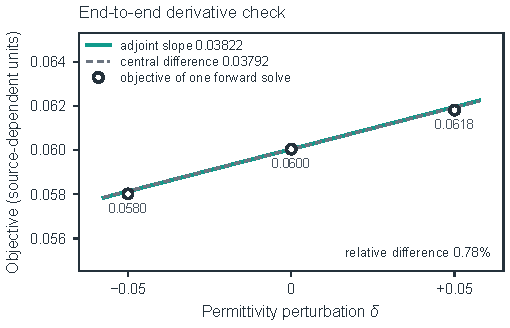
\includegraphics[width=0.56\linewidth]{figures/propagated-adjoint-check.pdf}
\caption{End-to-end derivative check of the fixed 44~\micron{} pillar-array objective on an RTX 3060. The objective is evaluated at the unperturbed and at two perturbed permittivities of the central pillar region, and the adjoint directional derivative and the central-difference secant are drawn as slopes through the unperturbed value. Both use one sampled output plane and propagation model.}
\label{fig:application}
\end{figure}

\section{Conclusion}

We have shown that the discrete adjoint of fused CUDA time stepping can be exposed to PyTorch and executed with its field state in host memory, so that a single workstation GPU returns material and geometry derivatives of full-wave photonic objectives. The transposed kernels of TorchFDTD give the gradient of differentiable Torch objectives built from the supported observations with respect to permittivity fields, densities, analytic solids, outlines and source waveforms, and its causal slab streaming bounds the device allocation by one slab and its halos while leaving the discrete problem unchanged. The package agrees with analytic solutions, Meep, FDTDX and a rigorous coupled-wave solver, and its adjoint matches automatic differentiation and finite differences. On the tested $64^3$ and $96^3$ scenes its full forward solves are 9.0 to 17.1 times faster than those of the package it extends on an A100 and \CrossFdtdxFullMin{} to \CrossFdtdxFullMax{} times faster than those of FDTDX on an RTX 3060. In double precision on the A100 they are \PrecisionRatioMin{} to \PrecisionRatioMax{} times faster than those of Meep on a workstation CPU. The software is available under the MIT license \citep{torchfdtd}.

Most remaining questions are architectural. First, host streaming keeps dense material arrays, state banks and checkpoints in host memory, so sustained optimization of a device whose field state exceeds the GPU will be governed by host capacity and device--host bandwidth, and the multi-GPU execution of one domain is the next step. Second, the tiled forward path invites a coupled formulation that recovers the lateral coupling that independent tiles discard. On the numerical side, dispersive media that cross an absorbing face and conformal treatment of curved metallic surfaces remain open. Within these bounds, the time-domain adjoint of a photonic device with tens of millions of cells can be evaluated on the hardware that a design group owns.

\section*{CRediT authorship contribution statement}

\textbf{Hyoseok Park:} Conceptualization, Methodology, Software, Validation, Formal analysis, Investigation, Data curation, Visualization, Writing -- original draft, Writing -- review and editing.

\section*{Funding}

\authorcheck{Funding statement to be completed by the author before submission. If the work received no specific grant, Elsevier recommends: This research did not receive any specific grant from funding agencies in the public, commercial, or not-for-profit sectors.}

\section*{Declaration of competing interest}

The author declares no competing financial interests or personal relationships that could have influenced the work reported in this paper.

\section*{Declaration of generative AI and AI-assisted technologies}

\textit{Software development.} During the development of TorchFDTD the author used generative AI tools (OpenAI GPT-6 Astra and Anthropic Claude Fable 5.1) for assistance with implementation, test generation and benchmark scripting. The resulting code was checked by the automated test suite and by the numerical validation reported in this work.

\textit{Manuscript preparation.} During the preparation of this manuscript the author used Anthropic Claude (Fable 5.1 and Opus 5.5) to improve the language, style and readability of the text. After using these tools the author reviewed and edited the content as needed and takes full responsibility for the content of the publication.

\section*{Data availability}

The source code, the test suite and the complete set of validation records are available in the public repository \citep{torchfdtd} and in the program files deposited with the CPC Program Library. Table~\ref{tab:gradients} and the remaining in-text values are taken from records in the repository. The A100 timing records were produced with the scripts in \code{benchmarks/a100_paper} of the repository, and the grid-size sweep, the microring field maps and the metagrating evaluation with those in \code{benchmarks/paper_review}. The drivers of the color-router cross-check are in \code{benchmarks/color_router_rcwa} of the repository, and the device model they require is in the repository of Ref.~\citep{park2026colorrouter}.

% elsarticle-num-names keeps the numbered style of elsarticle-num and also supplies author names for \citet.
\bibliographystyle{elsarticle-num-names}
\bibliography{references}

\end{document}
